\NeedsTeXFormat{LaTeX2e}
%-----------------------------------------------------------
\documentclass[a4paper,12pt]{monografia}
\usepackage[portuguese, colorinlistoftodos, textsize=tiny]{todonotes}
\usepackage{amsmath,amsthm,amsfonts,amssymb}
\usepackage[mathcal]{eucal}
\usepackage{latexsym}
\usepackage[portuguese]{babel}
\usepackage[utf8]{inputenc}
\usepackage{setspace}
\usepackage{tabularx}
%\usepackage{natbib}
\usepackage{bm}
\usepackage[portuguese,algoruled,longend, linesnumbered]{algorithm2e}
\usepackage{listings}
\usepackage{graphicx}
\usepackage{hyperref}
\hypersetup{colorlinks,
   debug=false,
   linkcolor=black,  %%% cor do tableofcontents, \ref, \footnote, etc
   citecolor=black,  %%% cor do \cite
   urlcolor=black,   %%% cor do \url e \href
   bookmarksopen=true,
}
\usepackage[alf,bibjustif]{abntex2cite}

\newcounter{todocounter}
\newcommand{\comment}[2][]
{\stepcounter{todocounter}\todo[caption={\thetodocounter: #2}, #1]
{\begin{spacing}{1}\thetodocounter: #2\end{spacing}}}
\reversemarginpar
\setlength{\marginparwidth}{2.5cm}
\lstloadlanguages{C}
%-----------------------------------------------------------
%-----------------------------------------------------------
\theoremstyle{plain}
\newtheorem{theorem}{Teorema}[section]
\newtheorem{axiom}{Axioma}[section]
\newtheorem{corollary}{Corol\'ario}[section]
\newtheorem{lemma}{Lema}[section]
\newtheorem{proposition}{Proposi\c{c}\~ao}[section]
%-----------------------------------------------------------
\theoremstyle{definition}
\newtheorem{definition}{Defini\c{c}\~ao}[section]
\newtheorem{example}{Exemplo}[section]
%-----------------------------------------------------------
\theoremstyle{remark}
\newtheorem{remark}{Observa\c{c}\~ao}[section]
%-----------------------------------------------------------
%-----------------------------------------------------------
\newcommand{\R}{\mathbb{R}}
\newcommand{\N}{\mathbb{N}}
\newcommand{\Z}{\mathbb{Z}}
\newcommand{\Q}{\mathbb{Q}}
\newcommand{\K}{\mathbb{K}}
\newcommand{\I}{\mathbb{I}}
\newcommand{\id}{\mathbf{1}}
\newcommand{\U}{\mathcal{U}}
\newcommand{\V}{{\cal V}}
%-----------------------------------------------------------
\def\ind{\hbox{ ind }}
%-----------------------------------------------------------
\hyphenation{Con-si-de-ra-mos}
\hyphenation{me-lhor}
\hyphenation{res-pos-ta}
\hyphenation{re-qui-si-tos}




\begin{document}
%%%%%%%%%%%%%%%%%%%%%%%%%%%%%%%%%%%%%%%%%%%%%%%%%%%%%%%%%%%5
%
%                  INFORMAÇÕES PRÉ-TEXTUAIS
%
%----------------- Título e Dados do Autor -----------------
\titulo{Utilizando Ontologias para apoiar a recomendação de revisores de código}
\autor{Vinicius Schettino} \nome{Vinicius} \ultimonome{Schettino}
%
%---------- Informe o Curso e Grau -----
\mestrado %Pode ser \bacharelado \licenciatura \especializacao \mestrado ou \doutorado
\curso{Engenharia de Software}
\dia{06} \mes{Setembro} \ano{2018} % data da aprovação
\cidade{Juiz de Fora}
%
%----------Informações sobre a Instituição -----------------
\instituicao{Universidade Federal de Juiz de Fora} \sigla{UFJF}
\unidadeacademica{Instituto de Ciências Exatas}
\departamento{Pós Graduação em Ciência da Computação}
%
%------Nomes do Orientador, 1o. Examinador e 2o. Examinador-
\orientador{Regina Braga}
\ttorientador{Doutora}
%

\maketitle






%--------Digite aqui o seu resumo em Portugu\^es--------------
\resumo{Resumo} As instru\c{c}\~oes aqui contidas objetivam auxiliar os autores na prepara\c{c}\~ao de documentos para impress\~ao de monografias do Departamento de Ci\^encia da Computa\c{c}\~ao. Os estilos encontram-se definidos em um modelo denominado Monografia.cls. O resumo deve ser escrito na mesma l\'ingua do texto (Portugu\^es, Ingl\^es ou Espanhol) e descreve o conte\'udo do texto em cerca de 150-200 palavras. Esta \'e a primeira vers\~ao das instru\c{c}\~oes e dos formatos e, portanto, sujeita a incorre\c{c}\~oes e omiss\~oes. Sugest\~oes de melhorias s\~ao muito benvindas: envie mensagem para jairo.souza@ufjf.edu.br.

\noindent \\ \textbf{Palavras-chave:} Monografia, latex, instru\c{c}\~oes.



%----Sum\'ario, lista de figura e de tabela ------------
 \tableofcontents \thispagestyle{empty} \listoffigures
\thispagestyle{empty} \listoftables \thispagestyle{empty}



\end{tabular}  \thispagestyle{empty}
%---------------------




%%%%%%%%%%%%%%%%%%%%%%%%%%%%%%%%%%%%%%%%%%%%%%%%%%%%%%%%%%%
%
%--------------In\'icio do Conte\'udo---------------------------
%
%
\pagestyle{ruledheader}
\chapter{Introdu\c{c}\~ao}

O \textit{code review} é considerado uma das principais técnicas para diminuição de defeitos de software \cite{Boehm2001}. Nela, o autor de uma alteração na base de código de um projeto submete tal conteúdo ao crivo de um conjunto de pares técnicos, que irão revisar sua estrutura com base em um lista de regras e convenções previamente definida. Diferentes aspectos relacionados ao autor, ao revisor e ao processo de revisão em si estão diretamente relacionados à eficiência da prática. Autores relatam a diminuição da incidência de \textit{anti-patterns} \cite{Kemerer2009} de acordo com o nível de participação dos envolvidos e cobertura do código revisado \cite{Meneely201437, Morales2015171, Bavota201581}. Reputação \cite{Baysal2013122, Bosu2014} e experiência \cite{Kononenko2015111} do revisor também parecem impactar nos efeitos do \textit{code review}

Intrinsecamente colaborativa, a atividade de \textit{code review} é exercida com suporte de ferramentas computacionais específicas \cite{Bacchelli2013}, principalmente no desenvolvimento distribuído. Dentro de workflows de trabalho descentralizados \cite{gousios2016}, a prática funciona como um \textit{gateway} de qualidade que busca garantir que apenas alterações aderentes aos padrões de qualidade do projeto serão incorporados à codebase principal. Esta etapa do desenvolvimento se torna uma oportunidade para disseminação de conhecimento, embate de ideias e discussão de melhores práticas entre profissionais de experiência e visões diferentes. Para tanto, percebe-se a necessidade de suporte computacional para essas atividades colaborativas.

Tais aspectos configuram o Desenvolvimento Distribuído de Software (DDS), onde equipes de desenvolvimento se encontram espalhadas por organizações e espaços geográficos distintos. Este novo ramo da Engenharia de Software vem modificando a relação entre empresas e sistemas, principalmente em relação às estratégias de negócios \cite{audy2007}. As próprias relações de negócios fomentam a distribuição das equipes, procurando diminuição dos custos e a incorporação de mão de obra qualificada que pode estar em qualquer lugar do planeta.

Neste contexto, porém, os os desafios à colaboração co-localizada são potencializados e as soluções tradicionais não são suficientes para fomentar esta aspecto das atividades distribuídas \cite{nicolaci2011}. Casey \cite{casey2010} mostra que, com a distribuição geográfica dos times, diversos outros desafios, antes considerados colaterais ou resolvidos, emergem de forma a ameaçar a colaboração entre os membros da equipe: barreiras culturais, temporais e geográficas; reengenharia dos processos de desenvolvimento; resistência em compartilhar informações e conhecimento com os pares distribuídos; entre outros desafios.

Estes desafios do Desenvolvimento Distribuído de Software afetam o \textit{code review} de duas formas distintas. Primeiro, o processo de revisão pode se tornar lento e ineficiente quando a colaboração é afetada, devido aos baixos níveis de participação e cobertura. O mesmo vale para a disseminação do conhecimento, que fica prejudicada. Outro desafio que se consolida é a escolha do revisor adequado para aquele \textit{patch}. Com um vasto número de opções e pouca informação disponível sobre seus aspectos técnicos e gerenciais (e.g. tempo disponível) já que não há contato co-localizado entre eles, a natureza distribuída deste tipo de desenvolvimento dificulta o processo de escolha do revisor, impactando negativamente a eficiência do processo.

Existem alguns trabalhos congêneres que demonstram métodos de recomendação de revisores \cite{yu2014,Xia2015261,jiang2017}. Esses trabalhos foram estudados e levados em consideração para escrita do presente texto. Também foram revisadas pesquisas que apontam caracterísitcas de revisões, revisores e autores que possivelmente potencializam a colaboração \cite{Kemerer2009,Bird2015191,Baysal2013122}.

As principais lacunas deixadas pelos trabalhos anteriores estão relacionadas aos objetivos e à avaliação dos métodos propostos, principalmente em DDS. Primeiramente, não há relato de método de recomendação de revisores de código com o objetivo específico de potencializar a colaboração. Por isso, métodos já propostos não utilizam métricas nem variáveis de entrada relacionadas aos aspectos de cooperação, coordenação e comunicação, como por exemplo a abordagem 3C em DDS \cite{fuks2003}.

Outro ponto observado diz respeito à avaliação dos modelos de avaliação. Os trabalhos encontrados se limitam a comparar seus resultados com métricas relacionadas à proximidade dos mesmos com a indicação manual do revisor. Ou seja, a eficência é tida de acordo com a interseção entre o recomendado automaticamente e por decisão de um especialista, geralmente um desenvolvedor. Este modelo assume que o responsável pela indicação manual tem os subsídios naturais para fazer uma boa escolha. Em DDS isso pode não ser verdade, uma vez que fatores como diferenças culturais, de horário, geográficas e de maturidade podem diminuir a compreensão do indicador e propiciar a escolha inadequada do revisor. Por isso, no contexto apresentado, outras formas de avaliação podem ser mais apropriadas. Trabalhos recentes em sistemas de recomendação atentam para a importância de outras métricas de avaliação, como transparência, desempenho e feedback dos usuários~\cite{he2016}.

Os métodos anteriormente propostos utilizam dados de expertise e reputação dos desenvolvedores para apontar os mais adequados para determinado conhecimento. São utilizados dados de proximidade de código ou de semântica com as revisões anteriores. Abordagens mais recentes de recomendação de revisores envolvem informações de colaboração, como por exemplo impacto do trabalho entre um revisor/autor no passado. Estas relaçẽs são geralmente modeladas como redes de colaboração e construídas através de análises semânticas de similaridade e frequência de colaboração entre determinados atores. Fu et al. \cite{fu2017} descreve uma recomendação baseada num grafo de relacionamento entre desenvolvedores e seu status de trabalho no projeto. Xia et al. \cite{xia2017} agrupa desenvolvedores utilizando métodos de proximidade para capturar relações implícitas e explícitas. Yu et al. \cite{yu2014,yu2014-2} estendem essa abordagem com métodos de aprendizado de máquina minerando os comentários para extrair metadados e enriquecer o modelo da rede colaborativa. Yang et al. \cite{yang2016} utilizam social network analysis (SNA) baseadas em informações de atividade recente dos potenciais revisores no projeto.

Como trabalhos recentes na área utilizam aspectos de redes colaborativas, buscamos aprofundar análises destas abordagens para propor novos métodos de recomendação que possam aumentar a eficiência da recomendação de revisores dentro do contexto escolhido.

Para aprimorar as abordagens colaborativas citadas, a simples rede colaborativa pode ser incrementada com informações relevantes, aumentando a eficiência de revisão e dos métodos de avaliação. Uma das formas angariar estas informações relevantes é através do uso de ontologias \cite{middleton2001,middleton2004}. A informações descobertas através das máquinas de inferência podem aumentar a eficiência do modelo de recomendação.

O uso de ferramentas computacionais para o processo de revisão de código se tornou prática comum nos últimos anos \cite{Bacchelli2013}. O GitHub é uma plataforma rica em repositórios de projetos de software. Muitos são de código aberto, disponíveis para mineração. São 24 milhões de usuários, 67 milhões de projetos e 47 milhões de revisões\footnote{https://octoverse.github.com/}, também chamadas de \textit{pull requests} no modelo de desenvolvimento ``\textit{pull based}'' \cite{gousios2014}.

Esta característica permitiu a extração e análise automatizadas das informações sobre as revisões em projetos de código aberto, através de APIs disponibilizadas para este fim. Foram extraídas métricas apontadas como relevantes para nossos objetivos pela literatura relacionada.

Assim, o objetivo deste trabalho é discutir como ontologias podem enriquecer uma rede colaborativa de desenvolvedores para apoiar na recomendação de revisores de código, propondo uma ontologia capaz de auxiliar no processo. A principal contribuição é a definição das informações relevantes e propor o modelo de extração destas das bases de dados disponíveis.

\textcolor{red}{\hl{-- ORGANIZAÇÃO DO TRABALHO --}}

\chapter{Referencial Teórico}

Este capítulo descreve os diferentes pressupostos teóricos necessários para entendimento do processo de recomendação de revisores. O contexto de desenvolvimento distribuído possui diversas variações quanto a processo e ferramentas, que são descritas nas seções seguintes.

\section{\textit{Code review}}\label{sec:code_review}
  O \textit{code review} é uma prática consolidada e difundida em diversas organizações, contemplando diferentes portes e segmentos de mercado. A técnica constitui da análise técnica de uma mudança a ser submetida à base principal de código (repositório-mestre) por parte de um revisor técnico, tendo como base uma lista de diretrizes e padrões a serem observados. As nuances do processo variam em cada contexto levando em consideração, por exemplo, tolerância a defeitos, modelo de desenvolvimento e os objetivos almejados.

\subsection{Relevância}\label{sec:relevancia}
  O \textit{code review} está associada diretamente à detecção precoce de defeitos em produtos de software \cite{schettino2014,Kemerer2009}, sendo reconhecida como uma das principais técnicas com este fim \cite{Boehm2001}. Mais especificamente, é relatada maior eficiência quanto aos defeitos não-funcionais, enquanto os defeitos funcionais são menos afetados no processo \cite{Beller2014202}. Outros autores reportam a diminuição de defeitos através de estudos de caso \cite{McIntosh2014192,Bavota201581,Morales2015171}.

\subsection{Histórico}\label{sec:historico}
  A atividade de revisão remonta da décade de 80 \cite{Fagan1976}, e desde então vem evoluindo para suportar interações mais rápidas e constantes, com uso de ferramentas computacionais e práticas ágeis. O Modern Code Review (MCR) surge em sinergia com os modelos ágeis e distribuídos de desenvolvimento, valorizando mais a comunicação e troca de experiências entre autor e revisor \cite{Bacchelli2013}.

\section{Pull Based Method}\label{sec:pull_based}
  O conceito de \textit{branches} é a base para sistemas de controle de versão descentralizados, como o  Git\footnote{https://git-scm.com/} e o Mercurial\footnote{https://www.mercurial-scm.org/}. Com as \textit{branches} é possível desenvolver paralelamente, submtendo e mesclando as alterações no código em momentos oportunos. Esta característica é interessante para o DDS, uma vez que o isolamento e a atomicidade do trabalho de cada um até o momento de submissão é fundamental para a coordenação dos esforços \cite{barr2012}.

  Estas tecnologias permitiram o surgimento de um paradigma de desenvolvimento baseado em pulls, ou \textit{pull-based method} \cite{gousios2014}. O processo de revisão de código evolui neste novo paradigma, servindo como um \textit{gateway} de qualidade que busca garantir que apenas alterações aderentes aos padrões de qualidade do projeto serão incorporados à codebase principal \cite{gousios2015}. A figura 1 ilustra tal modelo de trabalho instanciado no GitHub\footnote{https://github.com}, principal expoente que oferece este paradigma. Nele é representado um modelo comum em desenvolvimento OpenSource \cite{6385140}, onde há um \textit{core team} responsável por revisar os \textit{pulls} de seus colegas e da comunidade no geral. Neste modelo, a mudança chega à codebase principal somente se houver o aval de um membro do \textit{core team}.

   \begin{figure}[!htbp]
    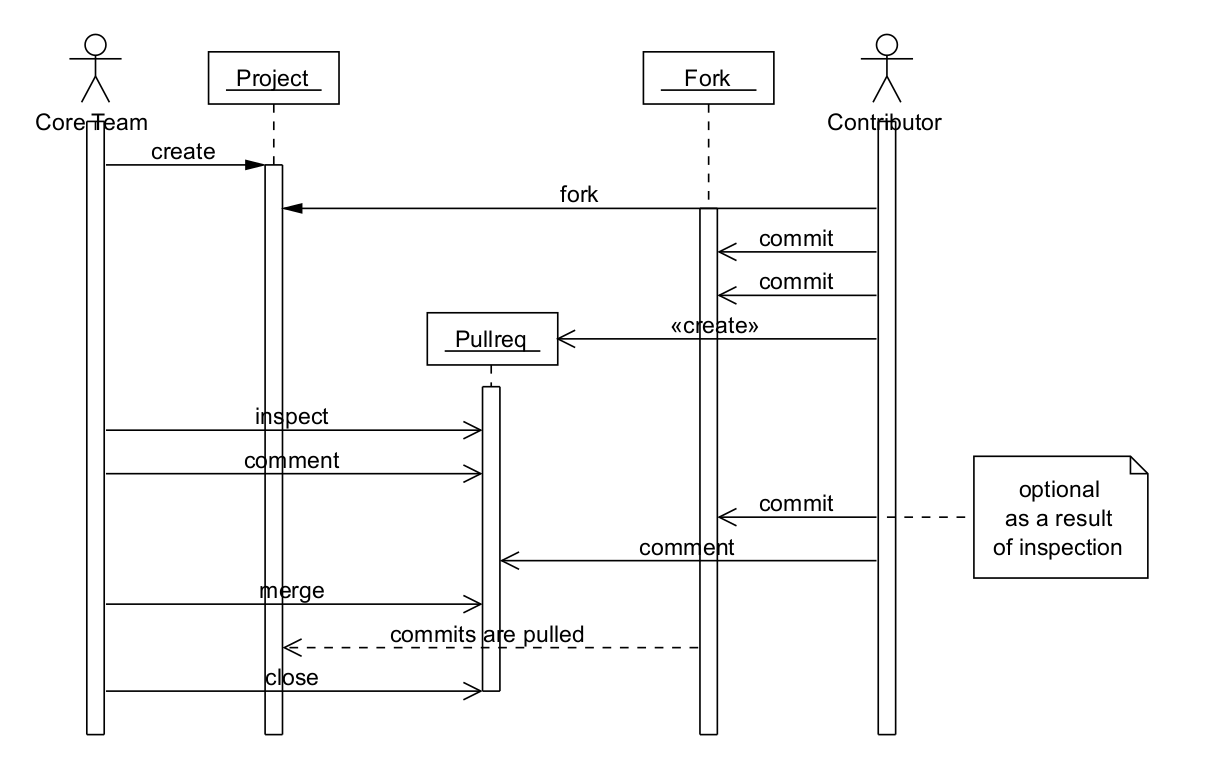
\includegraphics[width=\textwidth]{pull-request-flow}\label{fig:pull-request-flow}
    \caption{Pull Request Process \cite{gousios2014}}
  \end{figure}

  Aquele que deseja contribuir cria para si uma cópia do projeto através de um \textit{fork}. Esta ação cria em seu diretório de trabalho um projeto idêntico ao original, mas ao qual ele tem acesso total de submissão e modificação. Nessa cópia, ele executa as modificações desejadas, geralmente em uma \textit{branch} dedicada para tal \cite{gousios2016}. Ao terminar, ele solicita a integração da \texit{branch} do \textit{fork} de volta ao projeto original. Essa solitação é chamada de \textit{pull-request}, que será analisada por um desenvolvedor com as devidas permissões. Durante esta revisão, o autor pode gerar novas modificações, geralmente atreladas aos pedidos do revisor. Ao final, a mudança é rejeitada (\textit{closed}) ou aceita \textit{merged}.

  Os membros do core também têm suas \textit{branches} revisadas por um processo análogo \cite{6385140,Bosu2014}. A principal diferença é que não há necessidade do \texit{fork}, já que eles tem as permissões necessárias para criar uma nova \textit{branch} no projeto-alvo.

\section{Ontologia}

Ontologia é a definição de um vocabulário ou linguagem comum para representar conhecimentos \cite{gruber1995}. Para computação, pode ser vista como uma especificação formal, explícita e não ambígua de um conceito compartilhado por diferentes agentes.

As ontologias são utilizadas em diversos contextos e aplicações, geralmente com o objetivo de:

\begin{itemize}
  \item Compartilhar um conceito entre componentes de software.
  \item Reutilizar conceitos de um domínio em outro.
  \item Alinhar conceitos distintos propondo uma unificação explícita das diferentes visões.
\end{itemize}

uma ontologia é composta por: Definições de classes; Relações e Funções. Se tornou comum para representação de conhecimento na Web Semântica. As especificações da ontologia permitem a utilização de máquinas de inferências para descoberta de novos conhecimentos, antes não explícitos, nas informações disponíveis. Estas máquinas inferem novas propriedades e relacionamentos baseadas em conhecimento explícito \cite{berners2001}

\chapter{Trabalhos Relacionados}

Existem diversos trabalhos que visam recomendar revisores, alguns já citados em seções anteriores deste texto. Para esta seção foram escolhidos trabalhos fundamentais do campo, com atenção a diversidade de abordagens, especialmente no tocante da avaliação e métodos computacionais. O objetivo desta metodologia é oferecer uma visão ampla da área para identificar desafios e boas práticas que devem ser avaliados para proposta de novos métodos.

Balachandran \cite{balachandran2013} foi um dos primeiros autores a discutir a relevância da recomendação de revisores de código para o \textit{code review}. Ele propõe uma ferramenta não apenas para realizar uma série de análises para indicar modificações no código de maneira automatizada, mas também para encontrar o melhor revisor baseada em informações do \textit{changeset} em análise. A proposta também reconhece que em projetos muito grandes,  com muitos contribuidores, responsabilidades e código, é difícil que um ser humano possa, sem suporte, consolidar todas as informações necessárias para escolher um bom revisor.

É proposto então o ReviewBot, que utiliza as linhas alteradas no código e busca revisores que já atuaram no mesmo lugar. Estas informações são utilizadas para o revisor adequado, baseado em experiências passadas com aquele componente.

CoRReCT \cite{rahman2016} é uma ferramenta que também utiliza o histórico dos potenciais revisores para predição. Contudo, as informações em questão tangem a história dele como desenvolvedor. O especialista é definido pelas tecnologias com as quais ele trabalhou no passado, definidas como tópicos de conhecimento. A principal inovação da proposta é que o histórico completo do desenvolvedor, entre todas suas contribuições OpenSource que foram feitas no GitHub.

Para apoiar esta hipótese, foi conduzida uma análise exploratória. Os resultados indicam que várias bibliotecas e tecnologias são utilizadas em diversos projetos simultaneamente, e que por isso um especialista de um projeto pode ser de grande ajuda em outros também. É criada uma rede baseada em tópicos de conhecimento, para descoberta da expertise dos desenvolvedores em cada assunto.


cHRev \cite{zanjani2016} é outra abordagem que utiliza o histórico dos potenciais revisores. Contudo, aqui ao invés de encontrar através da similaridade do código, é analisado o quão participativo e útil ele foi em revisões passadas similares.

Esta análise é feita com base em três fatores: quantos comentários foram feitos, qual foi a velocidade de resposta e quão recente foi a revisão. Estas métricas servem para indicar o quão ativo foi o revisor anteriormente, fazendo dele alguém adequado para revisão em questão.

RevRec \cite{ouni2016} foca na expertise do desenvolvedor e analisa também as ocasiões de colaboração passada entre o desenvolvedor e o autor. A premissa é que uma relação passada positiva facilita a colaboração e pode evitar revisões ineficientes e tarefas manuais e custosas no processo.

Além disso, eles hipotetizam que é comum que autores busquem pares de revisão com os quais já trabalharam anteriormente para evitar conflitos. Por exemplo, evitam que criticas ou rejeições sejam interpretados como ofensas. Além de utilizar informações de atividade e utilidade do revisor em iterações passadas, esta abordagem busca analisar revisões semanticamente parecidas para recomendar.


Além de relevantes para o entendimento geral da área, os trabalhos selecionados também foram avaliados de acordo com a relevância do veículo de publicação e o fator de impacto QUALIS, como mostra a tabela~\ref{tab:presentation}. Os fatores constantes são oriundos da plataforma oficial da CAPES\footnote{https://sucupira.capes.gov.br/sucupira/public/consultas/coleta/veiculoPublicacaoQualis/listaConsultaGeralPeriodicos.jsf}


\begin{table}[!h]
\centering
\begin{tabularx}{\columnwidth}{|X|c|c|c|}
\toprule
\hline
Título                                                                                                                        & Ano & Fonte                               & Qualis &  \\
\hline
Reducing human effort and improving quality in peer code reviews using automatic static analysis and reviewer recommendation & 2013 & ICSE                                      & A1            &  \\
CoRReCT: code reviewer recommendation in GitHub based on cross-project and technology experience                             & 2016 & ICSE                                      & A1            &  \\
Automatically recommending peer reviewers in modern code review                                                              & 2016 & IEEE Transactions on Software Engineering & A1            &  \\
Search-Based Peer Reviewers Recommendation in Modern Code Review.                                                            & 2017 & ICSME                                  & A1            &  \\ \bottomrule
\hline

\end{tabularx}%
\caption{Chosen Papers Introduction}
\label{tab:presentation}
\end{table}


\chapter{Metodologia}

Os dados da análise são extraídos do GitHub através da API\footnote{https://developer.github.com/v3/} disponibilizada para desenvolvedores do mundo todo estenderem as funcionalidades da plataforma e integrar novos produtos que agregem valor ao processo de desenvolvimento. A versão estável para integração foi a v3, que implementa o padrão arquitetural RESTful\cite{fielding2002}. Existe a API em recém lançada v4\footnote{https://developer.github.com/v4/}, que utiliza da especificação GraphQL para exposição dos serviços. Esta não foi utilizada devido a documentação ainda recente e pela preferência ao padrão REST. A figura~\ref{fig:processo_extracao} mostra o pipeline de extração e estruturação dos dados.

\begin{figure}[!htbp]
 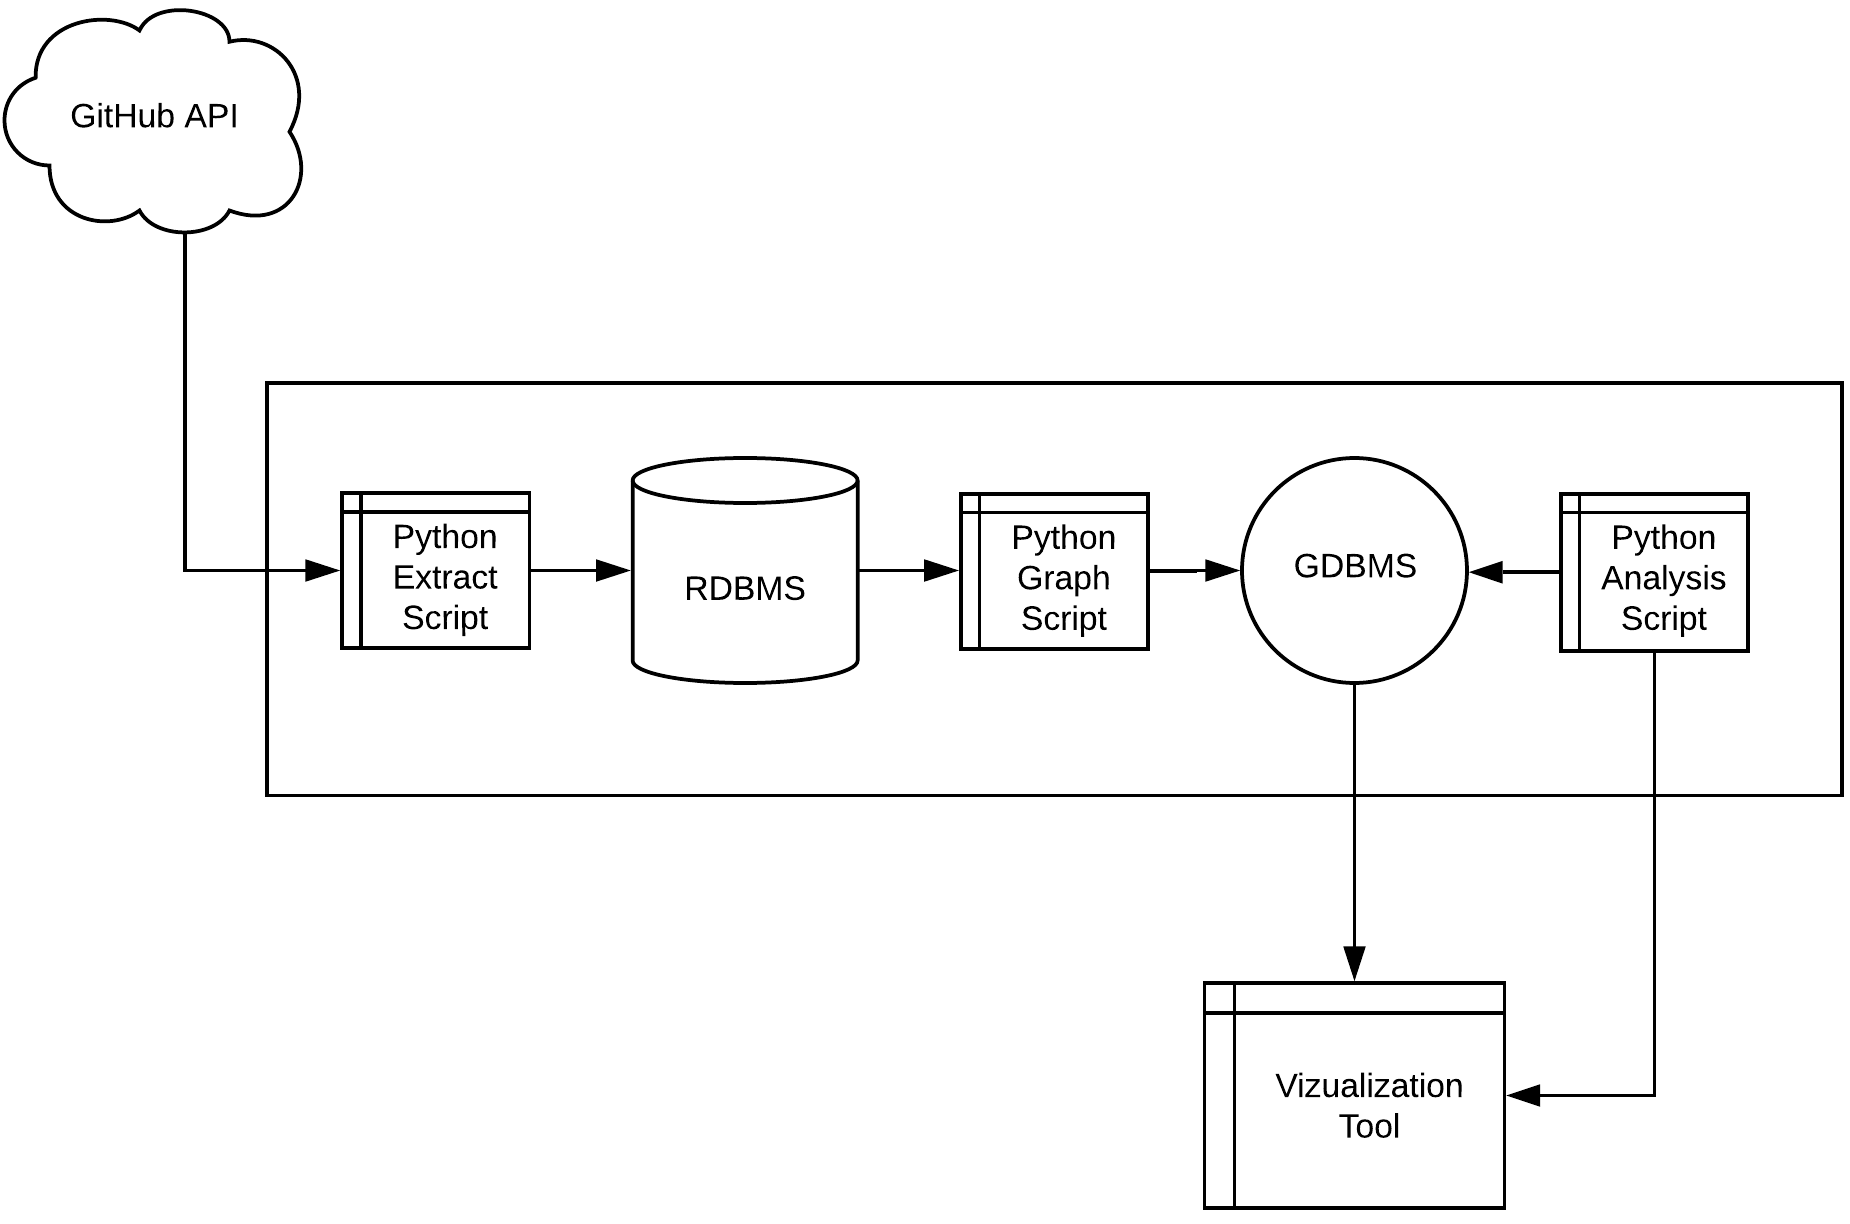
\includegraphics[width=\textwidth]{processo_extracao}
 \caption{Processo de extração dos dados}\label{fig:processo_extracao}
\end{figure}


Os dados extraídos são estruturados em um esquema relacional, mais especificamente em uma instância PostgreSQL 10.5. Este passo intermediário ocorre para que os dados fiquem disponíveis para outras análises, pesquisadores e ferramentas familiarizadas com o modelo relacional. Além disso, esta abordagem permite a extração de diversos metadados que não serão utilizados nas análises preliminares executadas na estrutura baseadas em grafo, ficando disponíveis para consultas posteriores sem degradar a performance do modelo em análise. A figura~\ref{fig:mer} mostra o modelo relacional proposto. As entidades \textit{user} são normalizadas entre os diferentes projetos. Ou seja, o usuário é uma entidade única que se relaciona a diferentes projetos, sem duplicação de seu conteúdo. Esta caracterísitca facilita futuras análises de colaboração entre projetos distintos. As \textit{labels} ligadas aos \textit{pullrequests} são utilizadas como descritores semânticos do conteúdo da contribuição, como por exemplo \textit{documentação}, \textit{python} ou \textit{performance}. As contribuições podem ser feitas através de comentários thread de discussão do \textit{pullrequests}, representados pelos \textit{discussioncomments} ou através dos de comentários no código em revisão, nos \textit{reviewcomments}. As \textit{reactions} são expressões de sentimento, ou \textit{emojis} utilizados para representar a opinião de maneira mais lúdica, como mostra a tabela ~\ref{fig:reactions}.

\begin{figure}[!htbp]
 \centering
 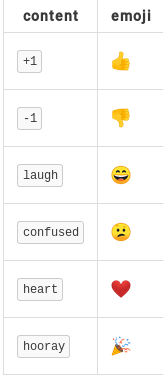
\includegraphics[height=150]{reactions}
 \caption{Tabela de Reactions Disponíveis}\label{fig:reactions}
\end{figure}

\begin{figure}[!htbp]
 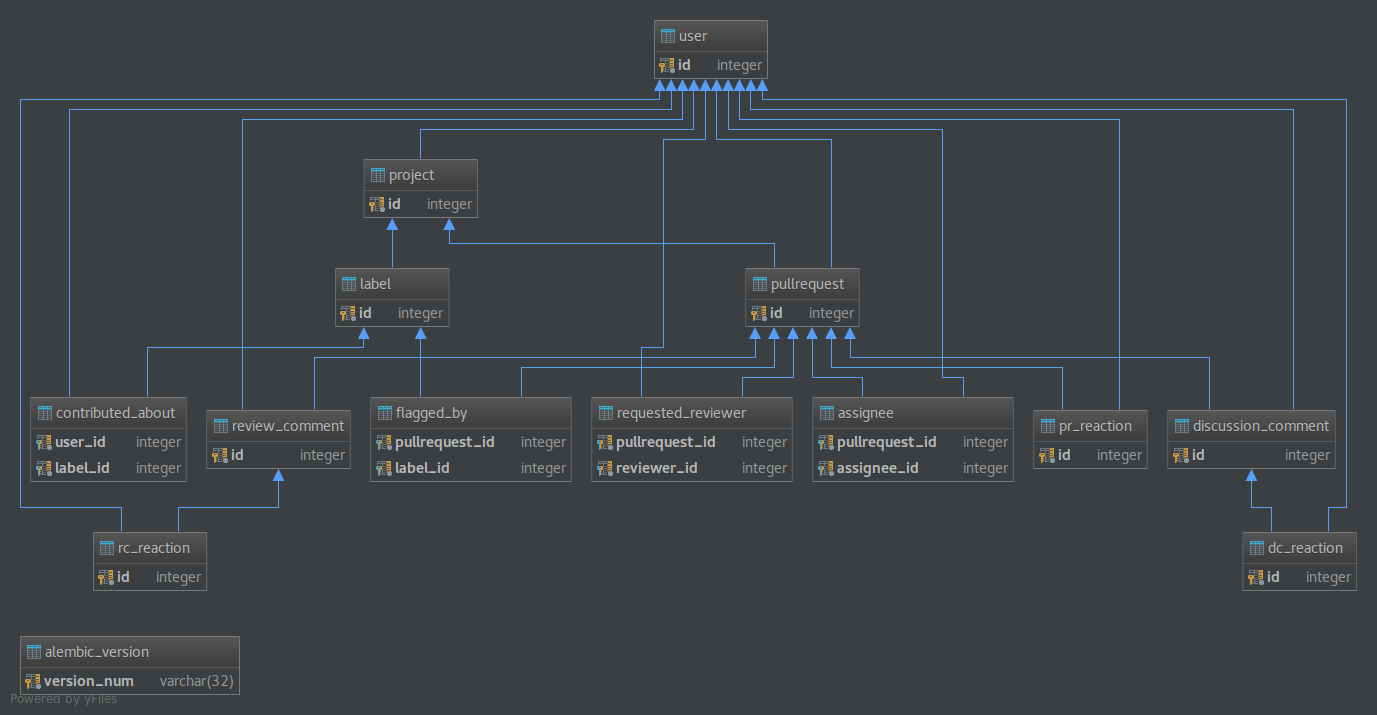
\includegraphics[width=\textwidth]{mer}
 \caption{Modelo Entidade Relacionamento}\label{fig:mer}
\end{figure}

Os dados são carregados para o banco de dados baseado em grafo (GDBMS), com as informações relevantes nos nós e arestas. Os dados de interesse são os autores e revisores, bem como o relacionamento entre eles. Detalhes da modelagem da rede colaborativa serão cobertos em uma seção específica. A tecnologia escolhida aqui é o Neo4j, banco de dados orientado a grafo mais popular de sua família\footnote{https://db-engines.com/en/ranking}. É a partir dele que as análises são executadas e vizualizadas utilizando o Gephi\footnote{https://gephi.org/}.

O algortimo de extração dos dados foi projetado com uma série de cuidados para garantir a integridade e disponibilidade das informações, diante das nuances do repostiório e do domínio de dados. Os principais aspectos observados são:

\paragraph{Inconsistência nos dados: } Para evitar dados inconsistentes, toda a extração é feita dentro de uma transaction relacional do SGBD, garantindo que todas as ações serão executadas (ou canceladas) de forma atômica. As restrições de chave primária também são a primeira linha de defesa para evitar que informações inconsistentes sejam armazenadas (como por exemplo um comentário relacionado a um pullrequest que não existe).

\paragraph{Tratamento das exceções da API: } O repositório de dados pode se comportar de maneira anormal durante a extração dos projetos, por diversos motivos: indisponibilidade dos serviços, lentidão do cliente, problemas de conexão entre outros. Assim é necessário tratar erros (como 400, 500 e 502) e evitar que o dump seja interrompido. Para isso, as respostas são tratadas, e detectados erros temporários como estes, o request é agendado para se repetir em uma janela de tempo definida.

\paragraph{Ratelimit da API: } A API do GitHub limita o número de requests a 5000/hora. Por isso, é necessário que o cliente controle o número de requests para que não seja bloqueado. Assim, o componente de extração limita o seu número de requests, entrando em espera quando o número se aproxima ao limite imposto.

\paragraph{Unicidade de usuários: } Usuários são entidades espalhadas entre os diferentes projetos. Para possibilitar análises globais e estatísticas realísticas de tamanhos de projetos, é necessário que não haja duplicação entre os usuários. O componente de extração também garante que não hajam usuários duplicados.



\section{Aspectos de Reprodutibilidade}

Cada uma das tecnologias apresentadas é encapsulada através da tecnologia de virtualização Docker. esta abordagem é uma resposta às iniciativas de reprodutibilidade na ciência, buscando maior transparência, confiabiliade e possibilidade de extensão nos experimentos \cite{freire2012}. Os três componentes (banco de dados relacional, orientado a grafo e os scripts de extração, transformação e carga) são encapsulados em contâiners distintos, como mostra a figur~\ref{fig:docker-model} Estes são orquestrados atravé do docker-compose, que configura os parâmetros e acessos necessários para o funcionamento do sistema sem que o usuário precise realizar nenhuma ação extra.

\begin{figure}[!htbp]
 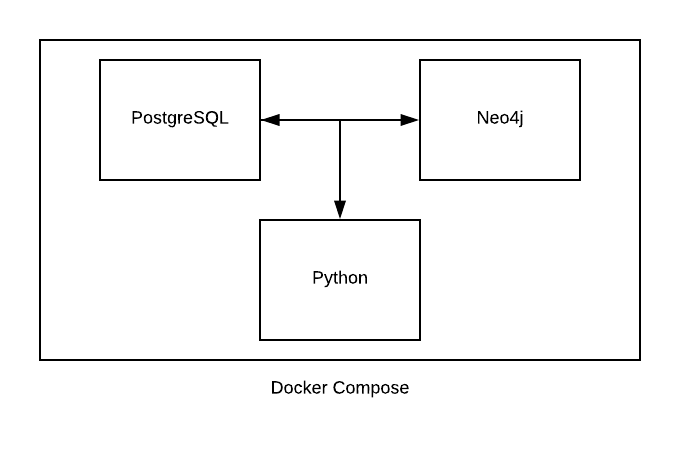
\includegraphics[width=\textwidth]{docker-model}
 \caption{Modelo de contâiners}\label{fig:docker-model}
\end{figure}


Com um conjunto grande de dependências, tecnologias e minúncias que estão envolvidas neste tipo de experimento, o código fonte e a descrição ainda que detalhada dos dados não é suficiente para alcançar níveis adequados de reprodutibilidade~\cite{ince2012}. Com auxílio dos containers Docker, é possível criar instâncias executáveis dos experimentos que vão funcionar em diferentes computadores, arquiteturas e situações, sem necessidade de conhecimento técnico por parte do executor das tecnologias utilizadas \cite{boettiger2015}.

De acordo com Sinha et al. \cite{sinha2016}, a maturidade da reprodutibilidade de um experimento científico computacional pode ser medido de acordo o nível dos seguintes aspectos que foram trabalhados em sua disponibilização. A figura~\ref{fig:espectro_reprodutibilidade} mostra o espectro de reprodutibilidade, que encara esta característica como um constante trabalho de evolução não binário, podendo uma pesquisa se tornar mais ou menos reprodutível ao se utilizar determinadas técnicas. A figura~\ref{fig:escala_reprodutibilidade} mostra o detalhamento de cada aspecto que contribui para que esta característica seja evidenciada:

\begin{figure}[!htbp]
 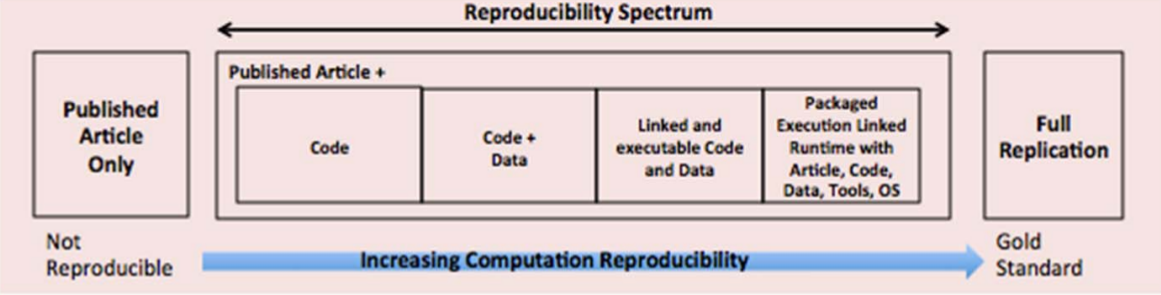
\includegraphics[width=\textwidth]{espectro_reprodutibilidade}
 \caption{Espectro de Reprodutibilidade}\label{fig:espectro_reprodutibilidade}
\end{figure}

\begin{figure}[!htbp]
 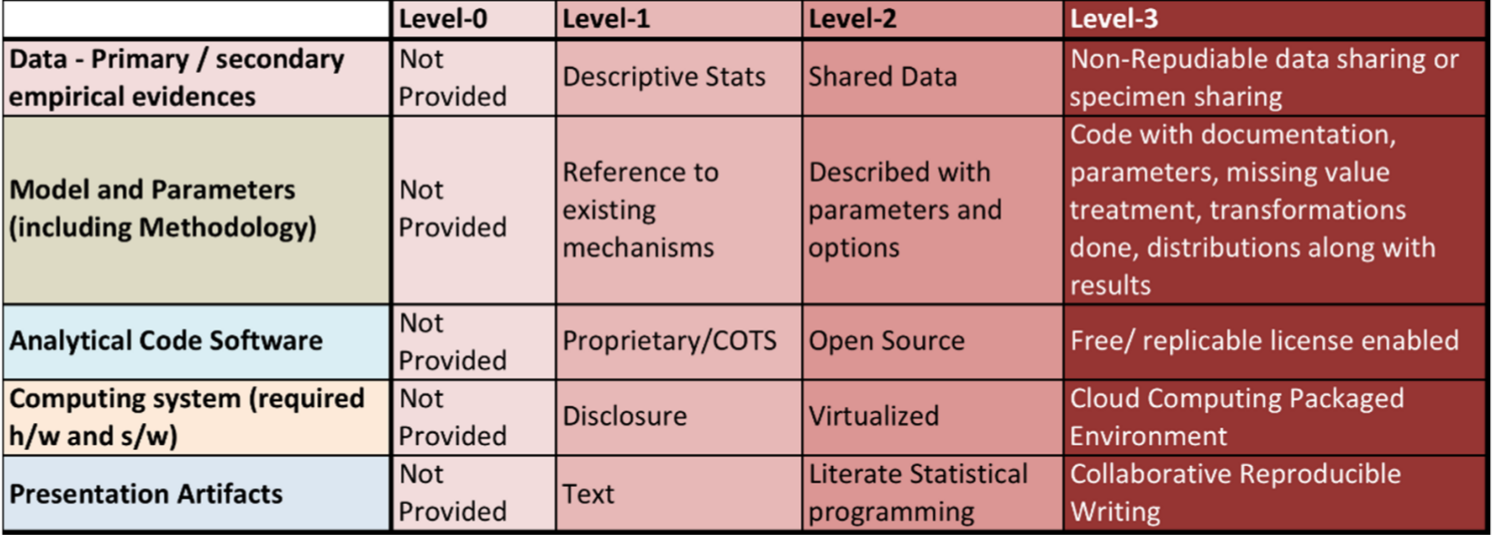
\includegraphics[width=\textwidth]{escala_reprodutibilidade}
 \caption{Escala de Maturidade de Reprodutibilidade}\label{fig:escala_reprodutibilidade}
\end{figure}


\paragraph{Dados - Evidências Primárias/Secundárias:} Análise da disponibilidade dos dados utilizados para futuros pesquisadores. Pode variar de simplesmente não dispobilizado até a disponibilização íntegra das informações, valendo-se de meios para uma oferta não repudiável e com garantias de integridade e veracidade. Neste trabalho, todos os dados (em suas diferentes agregações) são disponibilizados para uso futuro. Além disso os mecanismos de extração são automatizados, permitindo buscar outros projetos ou atualizar os dados dos já utilizados.

\paragraph{Modelo e Parâmetros:} Verificação dos modelos e parâmetros utilizados no experimento. São essenciais para a discussão e reprodução do experimento, além de qualquer tentativa de otimização. Varia de não disponibilizado até a disponibilização plena com documentação adequada, interface robusta que trate valores fora do domínio (como nulos) e também prática, facilitando os testes com parâmetros e dados distintos. Os modelos de dados e de execução são detalhados neste trabalho. Além disso, todas as análises são automatizadas e encapusladas através de comandos executáveis dentro de um contâiner Docker.

\paragraph{Código Fonte:} Disponibilidade do código fonte utilizado nas análises. Pode variar de não disponível (proprietário) até open source com direito de extensão e modificação. Neste projeto todo o código fonte é opensource e disponibilizado sob a permissiva licença MIT.

\paragraph{Sistema computacional requerido:} Detalhamento das informações de hardware e software necessários, como por exemplo memória, arquitetura, processador, versão e plataforma. O nível ideal é a disponibilização do experimento em ambiente virtualizado em nuvem, em arquitetura que permita tanto a reprodução "as is" quanto extensão e modificação de parâmetros e dados de entrada. Como todo o pipeline deste projeto está disponibilizado na infraestrutura Docker, a única restrição da máquina do pesquisador é ter o Docker instalado. Informações do hardware utilizado nos experimentos serão disponibilizadas nas próximas seções.


\section{Modelo Proposto}

O modelo proposto se baseia nos dados de relacionamento entre autores e revisores, mais espeficificamente nas interações entre comentários de revisão e pullrequests. Quanto existe uma interação do tipo, cria-se ou atualiza-se uma aresta entre dois indivíduos. A figura~\ref{fig:ger} ilustra o modelo proposto.

\begin{figure}[!htbp]
 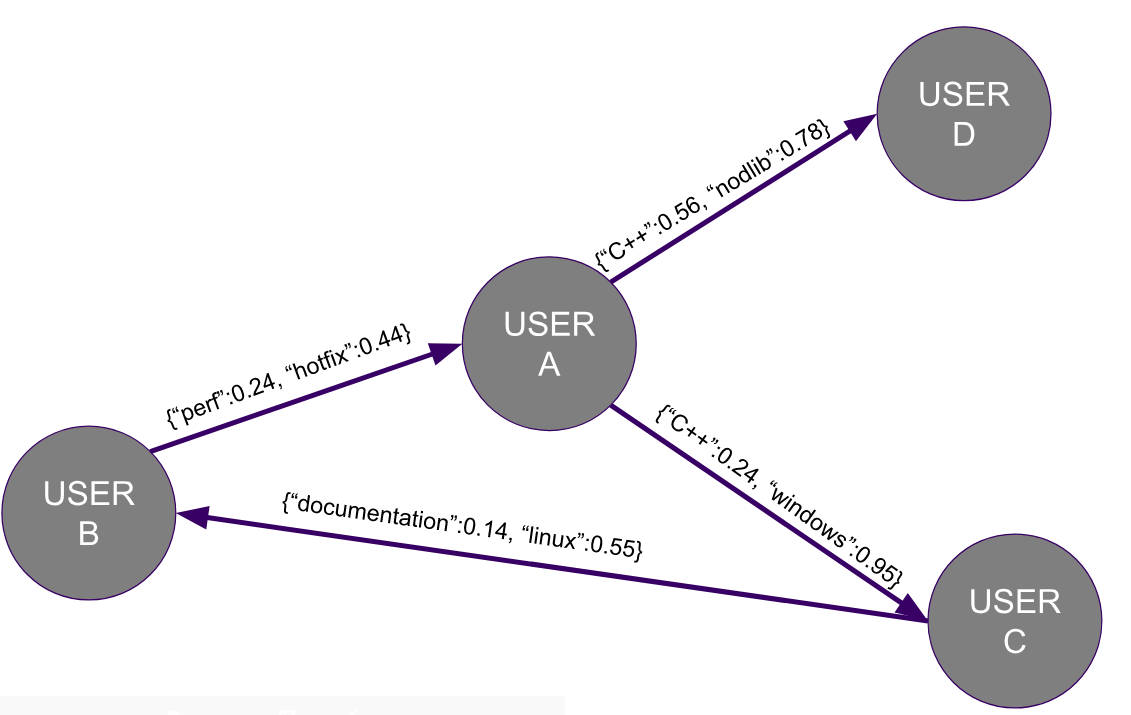
\includegraphics[width=\textwidth]{ger}
 \caption{Modelo da Rede Colaborativa}\label{fig:ger}
\end{figure}

O peso de cada aresta varia entre (0,1] e representa a importância que um revisor tem sobre determinado ator em determinado tópico de conhecimento. O tópico de conhecimento é definido através das labels de cada pullrequest. O cálculo é feito através da fórmula~\ref{eq:weight}.

\begin{equation}\label{eq:weight}
	W(A,B,label) = \dfrac{countRevs(A,B,tag)}{countTotRevs(B, tag)}.
\end{equation}

Para calcular o peso total do revisor A no autor B em determinada label, basta dividir a quantidade de revisões que A fez para B pelo total de revisões que B recebeu naquela label. Caso A tenha sido o único revisor naquele assunto, terá o peso máximo sobre ele neste contexto. Assim, este peso pode ser caracterizado como o nível influência que A têm sobre B.

Para facilitar a análise de métricas gerais de redes complexas, é introduzido ainda o peso médio de A sobre B, independente das tags. Ele é dado pela fórmula~\ref{eq:avg_weight}.

\begin{equation}\label{eq:avg_weight}
	avgW(A,B) = \dfrac{countRevs(A,B)}{countTotRevs(B)}.
\end{equation}

Este valor é utilizado para análises preliminares, por englobar um cenário geral sobre a relação entre os desenvolvedores.



\section{Escolha dos repositórios de dados}

Para avaliar as diferentes propriedades das redes colaborativas propostas, é necessário definir um conjunto de dados inseridos no contexto de estudo. As principais características buscadas foram:

\paragraph{Repositórios de GSD:} Como a recomendação de revisores têm maior relevância em desenvolvimento global de software, os repositórios escolhidos devem ser representantes deste contexto de desenvolvimento.

\paragraph{Acesso aberto: } Os repositórios devem estar disponíveis para uso em pesquisa e para futuras reproduções e extensões do estudo. Além disso há a restrição de estarem no GitHub para acesso via API.

\paragraph{Popularidade e Escala:} Os repostórios devem ser razoavelmente conhecidos e possuir um número de contribuidores que justifique a necessidade de recomendação de revisores. Para isso foram escolhidos projetos integrantes do top-10 "projects with the most reviews" eleitos pelo próprio GitHub\footnote{https://octoverse.github.com/}

A tabela~\ref{tab:repos} ilustra os projetos escolhidos e informações de contexto e tamanho.

\begin{table}[!h]
\centering
\resizebox{\textwidth}{!}{%
\begin{tabular}{@{}l|l|l|l|l|l|l@{}}
\toprule
\textbf{Nome} & \textbf{Linguagem Principal} & \textbf{Watchers} & \textbf{Stars} & \textbf{Contribuidores} & \textbf{Pull Requests} &  \\ \midrule\hline
Node.js    & JavaScript          & 2.868     & 52.709  & 2.088           & 8.440          &  \\
TensorFlow & C++/Python          & 8.293     & 108.249 & 1.624           & 8.562          &  \\
Kubernetes & Go                  & 2.675     & 40.610  & 1.776           & 41.059         &  \\
Symfony    & PHP                 & 1.297     & 18.381  & 1.692           & 17.475         &  \\ \bottomrule
\end{tabular}%
}
\caption{Descrição dos Respositórios Selecionados}
\label{tab:repos}
\end{table}

\section{Integração de repositórios de dados}

Apesar das ricas informações encontradas no GitHub, é possível refinar métodos de agrupamento e recomendação utilizando dados oriundos de outras fontes. Esta seção descreve a proposta de integração entre diferentes banco de dados para extrair informações relevantes para o modelo de rede colaborativa utilizado.

O StackOverflow é o maior site de Q&A (question and answer) aberto da web. A plataforma é anfitrã de milhões de perguntas e respostas, organizadas por tags administradas pela comunidade e por moderadores, sendo assim uma organização confiável quanto a relevância desta distribuição. Além disso, existem informações da pontuação dos envolvidos, bem como das respostas e perguntas realizadas. Este tipo de informação serve de proxy para descrever reputação dos participantes das discussões, especialmente inseridos no contexto de um conhecimento específico, como uma linguagem de programação ou framework.

Estas informações podem estender o poder de recomendação das abordagens baseadas na rede colaborativa apresentada, especialmente:


\begin{itemize}
  \item Refinando os resultados em caso de empates, através da Reputação.

  \item Refinando os agrupamentos baseado em mais informações de conhecimento, facilitando a colaboração.

  \item Mitigando problemas de \textit{cold start}, angariando mais informações sobre novos autores.
\end{itemize}

Contudo, tal integração não é trivial. Em bancos de dados distribuidos, diversos desafios são referenciados na literatura e impactam diretamente na eficiência e desempenho da integração \cite{ozsu2011}, notóriamente:

\paragraph{Meios de acesso heterogêneos:} Mesmo quando os dados estão semanticamente alinhados, os meios de acesso geralmente são distitos: APIs (RESTful, SOAP, etc), arquivos (XML/JSON) e SGBDs (relacional ou não, tecnologias distintas) raramente são facilmente compatíveis. Soluções de integração envolvem \textit{wrappers} que traduzem as nuances de cada repositório para uma interface homogênea que será acessada para as consultas globais.

\paragraph{Dados semanticamente conflitantes:} Muitas vezes entidades análogas são representadas com nomenclaturas diferentes, e o inverso também pode acontecer. O alinhamento destes domínios pode ser feito manualmente, através da sintática dos campos ou até utilizando estruturas de mediação, como as baseadas em ontologias.

\paragraph{\textit{matching} dos dados:} Mesmo quando há plena ciência, acesso e entendimento às diferentes bases, entidades análogas não necessariamente possuem dados idênticos. Pode haver falta de alguns dados ou até mesmo dados conflitantes. Para endereçar este problema, é necessário um processo de \texit{matching} que pode utilizar diferentes abordagens, que varia desde da comparação de atributos chave até a utilização de lógica \textit{fuzzy} para indicar tuplas correspondentes.

Outra discussão relevante é a forma de integração dos dados, que geralmente é divida em duas formas \cite{ozsu2011}: física ou lógica. O formato lógico consiste em disponibilizar uma interface homogênea virtual, onde as consultas globais são executadas. Estas são traduzidas e enviadas em tempo real para cada fonte de dados, e as respostas são integradas e apresentadas. Assim não existe união física das bases, e sim uma interface de consulta que permite consultas espalhadas nas diferentes fontes. Os principais problemas são as restrições de desempenho e a complexidade de distribuição das queries.

Outra abordagem consiste na consolidação dos dados distribuidos em uma única base, através de um processo conhecido como ETL (Extraction-Transform-Load). Os dados não são integrados em tempo real, mas sim em intervalos pré definidos. Esta característica faz com que o desempenho desta abordagem geralmente seja superior à integração lógica, e por isso é a base da maior parte dos datawarehouses e aplicações OLTP.

Buscando evitar a complexidade da distribuição de queries e visando flexibilidade nas transformações e no volume de dados em questão, optou-se pela abordagem física. Outros pesquisadores realizaram este tipo de integração com esta abordagem anteriormente, como descrito a seguir.

Para entender o impacto do StackOverflow no desempenho dos desenvolvedores, Vasilescu et al.~\cite{vasilescu2013} integram as bases para buscar correlação entre atividades nas plataformas e importância dos usuários. Para integrar as bases, sob a premissa de evitar falsos positivos, foi utilizada a técnica de correspondência completa entre emails das entidades "usuários" em ambas as bases de dados. A técnica deixa de fora usuários com mais de um email, reduzindo bastante o universo de dados resultante. Os repositórios dos dados são arquivos extraídos de forma offline de ambas as plataformas, criando um experimento que não pode ser facilmente atualizado ou a confecção de ferramenta que pode ser utilizada em tempo real.

De forma mais rebuscada, Silvestri et al.~\cite{silvestri2015} propõe uma integração entre três redes sociais: Twitter, StackOverflow e GitHub. Apesar de utilizar arquivos offline semelhantes à trabalhos anteriores (com adição da API REST do Twitter), o modelo de \textit{matching} é mais completo e tem potencial de encontrar mais correspondências corretas. Além de verificar o email, o perfil dos usuários é vasculhado para buscar referências aos perfis de outras redes. Além disso, informações como o login são utilizados tanto em correspondência direta quanto em correspondência parcial. A foto dos usuários também passa por um processo \textit{fuzzy} para indicar a probabilidade dos usuários serem os mesmos.

A abordagem aqui proposta une os principais aspectos positivos dos casos apresentados, adaptando aos objetivos da pesquisa e mitigando os principais defeitos. A primeira diferença é que no caso aqui descrito, existe uma base hierarquicamente mais relevante, de onde toda a informação estrutural da rede é extraída. No GitHub reside a maior parte da informação necessária, e por isso a extração é feita a partir dele. A integração com o StackOverflow é feita de maneira posterior e secundária, visando enriquecer as informações disponíveis para as análises.

Outro desafio que esta proposta precisa lidar de maneira mais eficiente é a atualização dos dados. Os modelos anteriores se baseiam em repositórios offlines que contém todas as informações de todos os projetos do GitHub. O objetivo aqui é propor uma ferramenta de recomendação viável, que possa ser recarregada com dados atualizados em tempo razoável para que recomendações precisas sejam feitas.

Assim, o modelo proposto extende a abordagem apresentada na seção 2, adicionando na extração dos dados do GitHub a busca no repositório de dados do StackOverflow, através da API\footnote{http://data.stackexchange.com/stackoverflow/queries} que implementa a interface SQL BigQuery\footnote{https://cloud.google.com/bigquery/public-data/stackoverflow}. As informações de cada usuários são então aprimoradas, como mostra a figura~\ref{fig:processo_extracao_stackoverflow}.


\begin{figure}[!htbp]
 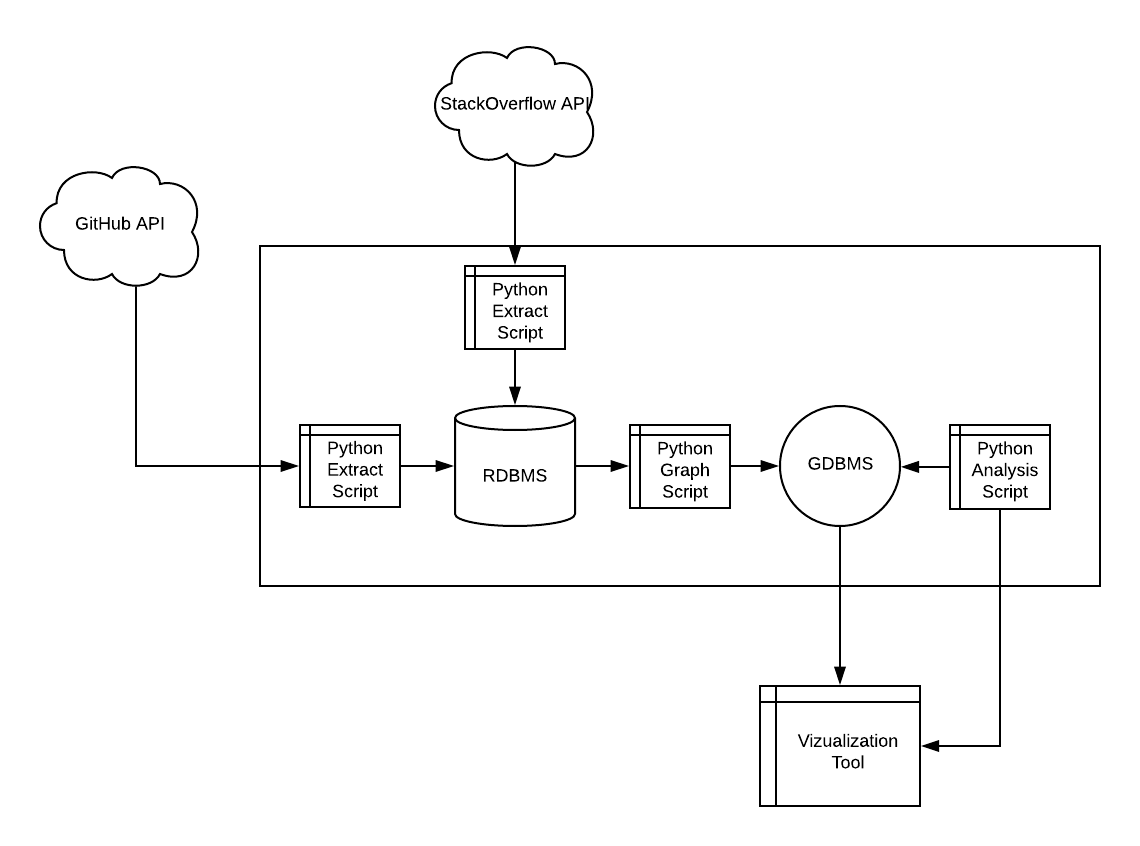
\includegraphics[width=\textwidth]{processo_extracao_stackoverflow}
 \caption{Processo de Extração com StackOverflow}\label{fig:processo_extracao_stackoverflow}
\end{figure}

Para o processo de matching, além das informações de email utilizadas anteriormente, pode-se utilizar a busca por referências ao perfil do StackOverflow no perfil do GitHub. Além disso o nome pode ser utilizado para \textit{matching} parcial e comparação com o login. Por exemplo, inferindo que \textit{John Smith} pode ser \textit{jsmith}. Para aumentar a precisão destes algoritmos, é possível também restringir as buscas aos usuários que façam menção ao projeto em processo de extração em seu perfil.

Dentre os principais dados relevantes para o processo de recomendação, estão aqueles relacionados a conhecimento e reputação dos usuários que estão também no StackOverflow. Os principais são:

\textit{informações de reputação: } É possível entender a presença do usuário no StackOverflow através da sua pontuação. Este \textit{score} é obtido através de diferentes formas de colaboração, como perguntas, respostas, reações, comentários e outras formas de interação. Usuários mais importantes para a rede tendem a ter pontuações mais altas. Este ranking pode ser utilizado para desempatar recomendações.

\textit{informações de conhecimento: } Analisar a contribuição dos potenciais revisores em determinadas áreas do conhecimento. Este rankeamento pode ser feito pelas tags do StackOverflow e serem comparadas com as informações semânticas de seu histórico no GitHub, como as labels ou tópicos extraídos do conteúdo dos pullrequests.



%%%%%%%%%%%%%%%%%%%%%%%%%%%%%%%%%%%%%%%
\singlespacing
\bibliographystyle{abntex2-alf}
\bibliography{../bibrefs/refs}

%%%%%%%%%%%%%%%%%%%%%%%%%%%%%%%%%%%%%%%%%%%%%%%%

\end{document}
